% !TeX TXS-program:compile = txs:///arara
% arara: pdflatex: {shell: yes, synctex: no, interaction: batchmode}
% arara: pdflatex: {shell: yes, synctex: no, interaction: batchmode} if found('log', '(undefined references|Please rerun|Rerun to get)')

\documentclass[a4paper]{article}
\usepackage[french]{babel}
\usepackage[utf8]{inputenc}
\usepackage[T1]{fontenc}
\usepackage{WriteOnGrid}
\usetikzlibrary{decorations.pathreplacing}
\usepackage{amsmath,amssymb}
\usepackage{fontawesome5}
\usepackage{enumitem}
\usepackage{frcursive}
\usepackage{lipsum}
\usepackage{tabularray}
\usepackage{fancyvrb}
\usepackage{fancyhdr}
\usepackage{frcursive}
\fancyhf{}
\renewcommand{\headrulewidth}{0pt}
\lfoot{\sffamily\small [WriteOnGrid]}
\cfoot{\sffamily\small - \thepage{} -}
\rfoot{\hyperlink{matoc}{\small\faArrowAltCircleUp[regular]}}

%\usepackage{hvlogos}
\usepackage{hologo}
\providecommand\tikzlogo{Ti\textit{k}Z}
\providecommand\TeXLive{\TeX{}Live\xspace}
\providecommand\PSTricks{\textsf{PSTricks}\xspace}
\let\pstricks\PSTricks
\let\TikZ\tikzlogo
\newcommand\TableauDocumentation{%
	\begin{tblr}{width=\linewidth,colspec={X[c]X[c]X[c]X[c]X[c]X[c]},cells={font=\sffamily}}
		{\huge \LaTeX} & & & & &\\
		& {\huge \hologo{pdfLaTeX}} & & & & \\
		& & {\huge \hologo{LuaLaTeX}} & & & \\
		& & & {\huge \TikZ} & & \\
		& & & & {\huge \TeXLive} & \\
		& & & & & {\huge \hologo{MiKTeX}} \\
	\end{tblr}
}

\usepackage{hyperref}
\urlstyle{same}
\hypersetup{pdfborder=0 0 0}
\usepackage[margin=1.5cm]{geometry}
\setlength{\parindent}{0pt}
\definecolor{LightGray}{gray}{0.9}

\def\TPversion{0.1.7}
\def\TPdate{01 septembre 2024}

\usepackage[most]{tcolorbox}
\tcbuselibrary{minted}
\NewTCBListing{PresentationCode}{ O{blue} m }{%
	sharp corners=downhill,enhanced,arc=12pt,skin=bicolor,%
	colback=#1!1!white,colframe=#1!75!black,colbacklower=white,%
	attach boxed title to top right={yshift=-\tcboxedtitleheight},title=Code \LaTeX,%
	boxed title style={%
		colframe=#1!75!black,colback=#1!15!white,%
		,sharp corners=downhill,arc=12pt,%
	},%
	fonttitle=\color{#1!90!black}\itshape\ttfamily\footnotesize,%
	listing engine=minted,minted style=colorful,
	minted language=tex,minted options={tabsize=4,fontsize=\footnotesize,autogobble},
	#2
}

\newcommand\Cle[1]{{\bfseries\sffamily\textlangle #1\textrangle}}

\begin{document}

\pagestyle{fancy}

\thispagestyle{empty}

\vspace{2cm}

\begin{center}
	\begin{minipage}{0.75\linewidth}
	\begin{tcolorbox}[colframe=yellow,colback=yellow!15]
		\begin{center}
			\begin{tabular}{c}
				{\Huge \texttt{WriteOnGrid [fr]}}\\
				\\
				{\LARGE Pour écrire sur les} \\
				{\LARGE lignes d'une grille.}
			\end{tabular}
			
			\medskip
			
			{\small \texttt{Version \TPversion{} -- \TPdate}}
		\end{center}
	\end{tcolorbox}
\end{minipage}
\end{center}

\vspace{0.5cm}

\begin{center}
	\begin{tabular}{c}
	\texttt{Cédric Pierquet}\\
	{\ttfamily c pierquet -- at -- outlook . fr}\\
	\texttt{\url{https://github.com/cpierquet/WriteOnGrid}}
\end{tabular}
\end{center}

\vspace{0.5cm}

{$\blacktriangleright$~~Quelques commandes créer une grille (5x5 ou Seyes ou Ruled) et écrire \og sur \fg{} les lignes.}

\smallskip

{$\blacktriangleright$~~Personnalisation de la taille de la grille, des marges, etc.}

\smallskip

{$\blacktriangleright$~~Possibilité de créer une page complète Seyes}

\vspace{1cm}

\begin{center}
	\begin{EnvQuadrillage}[NbCarreaux=22x8]
	\EcrireLigne{mon texte sur la ligne 1\ldots}
	\EcrireLigne<center>{mon texte centré sur la ligne 2\ldots}
	\EcrireLigne<right>{mon texte aligné à droite sur la ligne 3\ldots}
	\EcrireLigne[DecalH=2]{mon texte décalé de 2 carreaux sur la ligne 4\ldots}
	\PasseLigne
	\EcrireLigne{\sffamily mon texte sur la ligne 6\ldots}
	\EcrireLigne[DecalH=-1]{\small\cursive mon texte, décalé à gauche de 1 carreau, sur la ligne 7\ldots}
\end{EnvQuadrillage}
\end{center}

\begin{EnvQuadrillage}[NbCarreaux=24x5,Marge=1,Elargir=2/2,Grille=Seyes]<\CoulSeyes>
	\EcrireLigne[Echelle=1.5]{\textcolor{red}{mon texte sur la ligne 1\ldots}}
	\EcrireLigne[Echelle=1.5]{\textcolor{blue}{mon texte sur la ligne 2\ldots}}
	\EcrireLigne[Echelle=1.5,DecalH=-1]{$1+\frac{1}{2}=\frac32$ et $(1+x)^2=1+2x+x^2$ sur la ligne 3\ldots}
	\EcrireLigne[Echelle=1.5]{\cursive mon texte sur la ligne 4\ldots}
\end{EnvQuadrillage}

\vspace{0.5cm}

\hfill{}\textit{Merci à Patrick Bideault pour ses retours et idées !}

\vfill

\hrule

\medskip

\TableauDocumentation

\medskip

\hrule

\medskip

\newpage

\phantomsection
\hypertarget{matoc}{}

\tableofcontents

\newpage

\section{Le package WriteOnGrid}

\subsection{Chargement du package, packages utilisés}

Le package \textsf{WriteOnGrid} se charge dans le préambule via la commande :

\begin{PresentationCode}{listing only}
\usepackage{WriteOnGrid}
\end{PresentationCode}

Il est compatible avec les compilations usuelles en \textsf{latex}, \textsf{pdflatex}, \textsf{lualatex} ou \textsf{xelatex}.

\medskip

Pour des soucis de compatibilité, \texttt{xcolor} n'est pas chargé avec des options spécifiques, les couleurs utiles ont été définies directement dans le package.

\medskip

Il charge les packages et librairies suivantes :

\begin{itemize}
	%\item \texttt{xcolor} avec les options \Cle{table,svgnames} ;
	\item \texttt{tikz} avec les librairies \Cle{calc} et \Cle{positionning} ;
	\item \texttt{xstring} et \texttt{simplekv}.
\end{itemize}

\subsection{\og Philosophie \fg{} du package}

L'idée est de proposer, grâce à \TikZ, des \textsf{commandes} et \textsf{environnements} pour travailler sur un quadrillage et écrire \og sur les lignes \fg.

\begin{PresentationCode}{listing only}
%environnement francisé, avec clés en français pour préparer la grille
%commandes pour placer ou passer une ligne

\begin{EnvQuadrillage}[clés]<couleur(s)>
	\EcrireLigne[clés]<alignement>{texte}
	\PasseLigne
\end{EnvQuadrillage}
\end{PresentationCode}

\subsection{Fonctionnement global}

La grille est créée en spécifiant le nombre de carreaux (sous la forme nbCol$\times$nbLig), et on peut ensuite spécifier des \textit{débordements} latéraux pour éventuellement étendre le quadrillage dans les marges (gauche et droite). On peut également \textit{jouer} sur la marge, pour commencer les lignes à un niveau donné.

\medskip

Ci-dessous on représente une grille $5\times5$ :

\begin{itemize}
	\item de taille 24x5 ;
	\item avec un élargissement de \textcolor{red}{2 carreaux à gauche} et \textcolor{blue}{3 carreaux à droite} ;
	\item en commençant à écrire au niveau du \textcolor{orange}{1\up{er} carreau} ;
	\item un \textcolor{green!50!black}{\textit{cadre}} est rajouté pour visualiser la grille \textit{de base}.
\end{itemize}

\medskip

\begin{tikzpicture}
	\useasboundingbox (0,0) rectangle ({0.5*24},{-0.5*5}) ;
	\draw[xstep=0.5,ystep=0.5,thin,lightgray!50] ({-0.5*2},0) grid ({0.5*24+0.5*3},{-0.5*5}) ;
	\draw[thick,decorate,decoration={brace,amplitude=8pt,mirror}](0,{-0.5*5-0.25})--({0.5*24},{-0.5*5-0.25}) node[midway,below=8pt,font=\small\sffamily] {24C} ;
	\draw[red,thick,decorate,decoration={brace,amplitude=8pt,mirror}] ({-2*0.5},{-0.5*5-0.25})--({0},{-0.5*5-0.25}) node[midway,below=8pt,font=\small\sffamily] {2C} ;
	\draw[blue,thick,decorate,decoration={brace,amplitude=8pt,mirror}] ({0.5*24},{-0.5*5-0.25})--({0.5*24+3*0.5},{-0.5*5-0.25}) node[midway,below=8pt,font=\small\sffamily] {3C} ;
	\draw[thick,decorate,decoration={brace,amplitude=8pt}] ({0.5*24+3*0.5+0.25},0)--({0.5*24+3*0.5+0.25},{-0.5*5}) node[midway,right=8pt,font=\small\sffamily] {5C} ;
	\draw[very thick,orange,densely dashed] ({0.5*1},0)--({0.5*1},{-0.5*5}) ;
	\draw[green!50!black,thick] (0,0) rectangle ({0.5*24},{-0.5*5}) ;
\end{tikzpicture}

\vspace{1.5cm}

Il est à noter que le figure \texttt{tikzpicture} est \textit{délimitée} par le \textcolor{green!50!black}{\textit{cadre}}, afin de pouvoir gérer les débordements et l'alignement de l'environnement !

\smallskip

De plus, le bord gauche du \textcolor{green!50!black}{\textit{cadre}} est aligné sur la marge gauche de la page, donc la position du quadrillage dépend en partie de la configuration de \texttt{\textbackslash parindent}.

\pagebreak

\subsection{Couleurs prédéfinies}

Le package \textsf{WriteOnGrid} définit également des couleurs pour une saisie plus facile !

\begin{PresentationCode}{listing only}
\definecolor{TyrianPurple}{rgb}{0.4,0.01,0.24}
\definecolor{PapierRose}{HTML}{E6B8E6}
\definecolor{PapierGris}{HTML}{D7E2EE}
%Couleurs adaptées pour le Seyes
\def\CoulSeyes{PapierRose/PapierGris}
%Couleurs adaptées pour le Ruled
\def\CoulRuled{PapierGris/TyrianPurple}
\end{PresentationCode}

\begin{PresentationCode}{text only}
{\tikz \filldraw[TyrianPurple] (0,0) rectangle++ (6,1) node[midway,font=\bfseries\large,text=white] {\verb+TyrianPurple+};}

{\tikz \filldraw[PapierRose] (0,0) rectangle++ (6,1) node[midway,font=\bfseries\large,text=black] {\verb+PapierRose+};}

{\tikz \filldraw[PapierGris] (0,0) rectangle++ (6,1) node[midway,font=\bfseries\large,text=black] {\verb+PapierGris+};}
\end{PresentationCode}

\subsection{Le nombre de carreaux}

Le nombre de carreaux de la grille (pour les quadrillages individuelles et les environnements) peuvent être donnés de plusieurs manières :

\begin{itemize}
	\item \Cle{NbCarreaux=<nbcols>x<nblignes>} pour spécifier manuellement ;
	\item \Cle{NbCarreaux=Auto} pour remplir le reste de la page (horiz. et vert.) ;
	\item \Cle{NbCarreaux=Cx<nblignes} pour remplir horizontalement et spécifier le nombre de lignes ;
	\item \Cle{NbCarreaux=<nbcols>xL} pour remplir verticalement et spécifier le nombre de colonnes.
\end{itemize}

À noter que les calculs effectués pour déterminer la \textit{place} restante ne tiennent pas compte des éventuels ressorts élastiques que \LaTeX\ peut rajouter pour \textit{optimiser} la place.

\smallskip

Pour \textit{forcer} l'ajout de ligne(s) supplémentaire(s), il est possible d'utiliser :

\begin{itemize}
	\item \Cle{NbCarreaux=Auto*} pour forcer l'ajout d'une ligne en plus ;
	\item \Cle{NbCarreaux=Auto**} pour forcer l'ajout de deux lignes en plus ;
	\item \Cle{NbCarreaux=Auto***} pour forcer l'ajout de trois lignes en plus ;
	\item etc
\end{itemize}

\pagebreak

\section{Grilles individuelles}

\subsection{La commande}

\begin{PresentationCode}{listing only}
%commande francisée, avec clés en français pour préparer la grille

\AffQuadrillage[clés]<couleur(s)>
\end{PresentationCode}

Le premier argument, \textit{optionnel}, entre \texttt{[...]} propose les \Cle{clés} :

\begin{itemize}
	\item \Cle{NbCarreaux} pour spécifier le nombre de carreaux, sous la forme \texttt{(nbCol)x(nbLig)} ; \hfill~défaut : \Cle{17x5}
	\item \Cle{Unite} pour spécifier l'échelle de la figure ; \hfill~défaut : \Cle{1}
	\item \Cle{Marge} pour spécifier la \textcolor{orange}{marge} du début des lignes ; \hfill~défaut : \Cle{0}
	\item le booléen \Cle{AffBarre} pour afficher ou non la marge ; \hfill~défaut : \Cle{true}
	\item \Cle{Elargir} pour préciser les carreaux de débordements, sous la forme unique \texttt{\textcolor{red}{G}\textcolor{blue}{D}} ou par côté \texttt{\textcolor{red}{G}/\textcolor{blue}{D}} ;\hfill~défaut : \Cle{0}
	\item le booléen \Cle{Cadre} pour afficher le cadre de base du quadrillage ;\hfill~défaut : \Cle{false}
	\item la clé \Cle{Grille}, parmi \Cle{5x5 / Seyes / Ruled}, pour spécifier le type de quadrillage ;\hfill~défaut : \Cle{5x5}
	\item la clé \Cle{ReglureSeyes} pour paramétrer (en mm) la réglure dans le cas de lignes Seyes ;\hfill~défaut : \Cle{2}
	\item la clé \Cle{CouleurBarreSeyes} pour rajouter un trait vertical pour le papier Seyes .\hfill~défaut : \Cle{red!75}
\end{itemize}

Le second argument, \textit{optionnel}, entre \texttt{<...>} correspond quant à lui à la couleur de base du quadrillage :

\begin{itemize}
	\item sous la forme \Cle{Couleur} (\Cle{lightgray!50} par défaut) pour le quadrillage $5\times5$ ;
	\item sous la forme \Cle{CouleurP/CouleurS} (\Cle{lightgray!50/lightgray!25} par défaut) pour le Seyes ou le Ruled.
\end{itemize}

\medskip

\begin{PresentationCode}{listing only}
%18x4 grands carreaux, sans dépassement, couleurs adaptées, sans marge/barre
\AffQuadrillage[NbCarreaux=16x4,Grille=Seyes,ReglureSeyes=2.5,AffBarre=false]<\CoulSeyes>

%36x8 petits carreaux, avec débordements 3/3, couleur PapierGris
\AffQuadrillage[NbCarreaux=36x6,Elargir=3/3]<PapierGris>

%12x3 lignes "Ruled", sans débordements, couleur Ruled, centré, avec marge
\begin{center}
	\AffQuadrillage[NbCarreaux=12x3,Elargir=2/2,Grille=Ruled,Marge=2]<\CoulRuled>
\end{center}
\end{PresentationCode}

\medskip

\AffQuadrillage[NbCarreaux=18x4,Grille=Seyes,ReglureSeyes=2.5,AffBarre=false]<\CoulSeyes>

\medskip

\AffQuadrillage[NbCarreaux=36x8,Elargir=3/3]<PapierGris>

\begin{center}
	\AffQuadrillage[NbCarreaux=12x3,Elargir=2/2,Grille=Ruled,Marge=2]<\CoulRuled>
\end{center}

\pagebreak

\subsection{L'environnement}

\begin{PresentationCode}{listing only}
%environnement francisé, avec clés en français pour préparer la grille

\begin{EnvQuadrillage}[clés]<couleur(s)>
	...
\end{EnvQuadrillage}
\end{PresentationCode}

Le premier argument, \textit{optionnel}, entre \texttt{[...]} propose les \Cle{clés} :

\begin{itemize}
	\item \Cle{NbCarreaux} pour spécifier le nombre de carreaux, sous la forme \texttt{(nbCol)x(nbLig)} ; \hfill~défaut : \Cle{17x5}
	\item \Cle{Unite} pour spécifier l'échelle de la figure ; \hfill~défaut : \Cle{1}
	\item \Cle{Marge} pour spécifier la \textcolor{orange}{marge} du début des lignes ; \hfill~défaut : \Cle{0}
	\item le booléen \Cle{AffBarre} pour afficher ou non la marge ; \hfill~défaut : \Cle{true}
	\item \Cle{Elargir} pour préciser les carreaux de débordements, sous la forme unique \texttt{\textcolor{red}{G}\textcolor{blue}{D}} ou par côté \texttt{\textcolor{red}{G}/\textcolor{blue}{D}} ;\hfill~défaut : \Cle{0}
	\item le booléen \Cle{Cadre} pour afficher le cadre de base du quadrillage ;\hfill~défaut : \Cle{false}
	\item la clé \Cle{Grille}, parmi \Cle{5x5 / Seyes / Ruled}, pour spécifier le type de quadrillage ;\hfill~défaut : \Cle{5x5}
	\item la clé \Cle{ReglureSeyes} pour paramétrer (en mm) la réglure dans le cas de lignes Seyes ;\hfill~défaut : \Cle{2}
	\item la clé \Cle{CouleurBarreSeyes} pour rajouter un trait vertical pour le papier Seyes .\hfill~défaut : \Cle{red!75}
\end{itemize}

Le second argument, \textit{optionnel}, entre \texttt{<...>} correspond quant à lui à la couleur de base du quadrillage :

\begin{itemize}
	\item sous la forme \Cle{Couleur} (\Cle{lightgray!50} par défaut) pour le quadrillage $5\times5$ ;
	\item sous la forme \Cle{CouleurP/CouleurS} (\Cle{lightgray!50/lightgray!25} par défaut) pour le Seyes ou le Ruled.
\end{itemize}

\medskip

\begin{PresentationCode}{listing only}
%des cadres ont été rajoutés pour la sortie

%18x4 grands carreaux, sans dépassement, couleurs adaptées, marge de 3 carreaux
\begin{EnvQuadrillage}[NbCarreaux=18x4,Grille=Seyes,Marge=3]<\CoulSeyes>
\end{EnvQuadrillage}

%36x8 petits carreaux, avec débordements 3/3, couleur PapierGris
\begin{EnvQuadrillage}[NbCarreaux=36x8,Elargir=3/3]<PapierGris>
\end{EnvQuadrillage}

%12x3 lignes "Ruled", sans débordements, couleur Ruled, centré, avec marge
\begin{center}
	\begin{EnvQuadrillage}[NbCarreaux=12x3,Elargir=2/2,Grille=Ruled,Marge=2]<\CoulRuled>
	\end{EnvQuadrillage}
\end{center}
\end{PresentationCode}

\medskip

\begin{EnvQuadrillage}[NbCarreaux=18x4,Grille=Seyes,Marge=3]<\CoulSeyes>
\end{EnvQuadrillage}

\smallskip

\begin{EnvQuadrillage}[NbCarreaux=36x8,Elargir=3/3,Cadre]<PapierGris>
\end{EnvQuadrillage}

\begin{center}
	\begin{EnvQuadrillage}[NbCarreaux=12x3,Grille=Ruled,Marge=2]<\CoulRuled>
\end{EnvQuadrillage}
\end{center}

\pagebreak

\subsection{Écrire sur les lignes}

L'idée est maintenant de pouvoir écrire sur les lignes du quadrillage créé (environnement !), et pour garantir le fait d'écrire \textit{pile} sur le ligne, on applique les recommandations suivantes :

\begin{itemize}
	\item les lignes doivent être saisies une par une, du \og haut \fg{} vers le \og bas \fg{} ;
	\item pas de paragraphe \textit{multilignes}, pas de puce ou de numérotation ;
	\item une ligne peut être passée.
\end{itemize}

\begin{PresentationCode}{listing only}
...
	%pour saisir les lignes, une par une
	\EcrireLigne[clés]<alignement>{texte}
	%pour passer la ligne
	\PasseLigne
...
\end{PresentationCode}

Le premier argument, entre \texttt{[...]} propose les \Cle{clés} :

\begin{itemize}
	\item \Cle{DecalH} pour spécifier le décalage horizontal (en carreaux) de la ligne, par rapport à la \textcolor{orange}{marge} ; \hfill~défaut : \Cle{0}
	\item \Cle{DecalV} pour spécifier le décalage vertical du texte par rapport à la ligne ; \hfill~défaut : \Cle{0pt}
	\item \Cle{Echelle} pour spécifier l'échelle du texte à écrire.\hfill~défaut : \Cle{1}
\end{itemize}

Le deuxième argument, \textit{optionnel}, entre \texttt{<...>} permet de spécifier l'alignement horizontal (parmi \Cle{left/center/right}) du texte dans le \textcolor{green!50!black}{\textit{cadre}} de base, \Cle{left} par défaut.

\medskip

Le troisième argument, \textit{obligatoire} et entre \texttt{\{...\}} est quant à lui le texte à saisir, avec possibilité de spécifier taille, couleur, fonte, etc

\begin{PresentationCode}{listing only}
\begin{EnvQuadrillage}[NbCarreaux=36x8]
	\EcrireLigne{mon texte sur la ligne 1\ldots}
	\EcrireLigne[Echelle=1.25]<center>{\ttfamily mon texte, en fonte teletype +25\,\%, centré sur la ligne 2\ldots}
	\EcrireLigne<right>{mon texte aligné à droite sur la ligne 3\ldots}
	\EcrireLigne[DecalV=0.1]{\textcolor{red}{mon texte rouge sur la ligne 4, décalé de 1mm vers le haut\ldots}}
	\PasseLigne
	\EcrireLigne[Echelle=0.5]{\sffamily mon texte, en fonte sans réduite de 50\,\%, sur la ligne 6\ldots}
	\EcrireLigne[DecalH=3]{\cursive mon texte sur la ligne 7, décalé de 3 carreaux\ldots}
\end{EnvQuadrillage}
\end{PresentationCode}

\begin{EnvQuadrillage}[NbCarreaux=36x8]
	\EcrireLigne{mon texte sur la ligne 1\ldots}
	\EcrireLigne[Echelle=1.25]<center>{\ttfamily mon texte, en fonte teletype augmentée de 25\,\%, centré sur la ligne 2\ldots}
	\EcrireLigne<right>{mon texte aligné à droite sur la ligne 3\ldots}
	\EcrireLigne[DecalV=0.1]{\textcolor{red}{mon texte rouge sur la ligne 4, décalé de 1mm vers le haut\ldots}}
	\PasseLigne
	\EcrireLigne[Echelle=0.5]{\sffamily mon texte, en fonte sans réduite de 50\,\%, sur la ligne 6\ldots}
	\EcrireLigne[DecalH=3]{\cursive mon texte sur la ligne 7, décalé de 3 carreaux\ldots}
\end{EnvQuadrillage}

\begin{PresentationCode}{listing only}
\begin{EnvQuadrillage}[NbCarreaux=22x4,Marge=2,Elargir=2/3,Grille=Seyes]
	\EcrireLigne[Echelle=1.5]{\textcolor{red}{mon texte rouge, un peu agrandi, sur la ligne 1\ldots}}
	\EcrireLigne[Echelle=1.15,DecalH=1]{$(1+x)^2=1+2x+x^2$ sur la l2, avec un décal de 1 en plus\ldots}
	\EcrireLigne[DecalH=-1.75]{\textcolor{blue}{mon texte bleu, remis un peu à gauche, sur la ligne 3\ldots}}
\end{EnvQuadrillage}

\end{PresentationCode}
\begin{EnvQuadrillage}[NbCarreaux=22x4,Marge=2,Elargir=2/3,Grille=Seyes]
	\EcrireLigne[Echelle=1.5]{\textcolor{red}{mon texte rouge, un peu agrandi, sur la ligne 1\ldots}}
	\EcrireLigne[Echelle=1.15,DecalH=1]{$(1+x)^2=1+2x+x^2$ sur la ligne 2, avec un décalage de 1 carreau en plus\ldots}
	\EcrireLigne[DecalH=-1.75]{\textcolor{blue}{mon texte bleu, remis un peu à gauche, sur la ligne 3\ldots}}
\end{EnvQuadrillage}

\pagebreak

\section{Page complète type Seyes}

\subsection{Idée et fonctionnement global}

Il s'agit ici de créer le quadrillage Seyes sur la page complète, comme pour la copie d'un élève !

Il est possible de paramétrer le type de papier (A4, A5 ou Lxh), et les marges sont adaptées automatiquement pour coller au type de papier.

\smallskip

\faBomb{} Le fonctionnement est différent des environnements \textit{ponctuels} précédents, et l'écriture sur les lignes du quadrillage peuvent poser souci avec des environnements mathématiques !!

\medskip

La grille complète est liée à un environnement (basé sur \texttt{tikzpicture}), et les commandes pour écrire sont à mettre dans l'environnement.

\smallskip

Tout le placement est géré grâce à un point (fictif), nommé \texttt{(SeyesOrigine)}, qui correspond au point de départ de l'écriture sur la copie !

\begin{PresentationCode}{listing only}
\begin{PleinePageSeyes}[options]
	\LignePapierSeyes[options]<alignement>(ajustement){texte}
	\CadreNoteSeyes[hauteur]{numligne}
	\ParagraphePapierSeyes[options]<alignement>(ajustement){texte}
\end{PleinePageSeyes}
\end{PresentationCode}

\subsection{La grille}

Pour l'environnement de création de la grille, l'argument, \textit{optionnel} et entre \texttt{[...]}, propose :

\begin{itemize}
	\item la clé \Cle{CouleurP} pour la couleur des \textit{gros traits} ;\hfill~défaut : \Cle{PapierRose}
	\item la clé \Cle{CouleurS} pour la couleur des \textit{petits traits} ;\hfill~défaut : \Cle{PapierGris}
	\item la clé \Cle{CouleurMarge} pour la couleur du trait de la marge ;\hfill~défaut : \Cle{red!75}
	\item le booléen \Cle{NumLignes} pour afficher le numéro des lignes (pour aider !) ; \hfill~défaut : \Cle{false}
	\item la cle \Cle{ReglureSeyes} pour spécifier la réglure, en mm ;\hfill~défaut : \Cle{2}
	\item la cle \Cle{FormatPapier} parmi \Cle{A4 / A5 / lxh}. \hfill~défaut : \Cle{A4}
\end{itemize}

\subsection{La commande pour saisir une ligne}

La commande \texttt{LignePapierSeyes} permet de saisir une ligne \textbf{unique}, un peu comme la commande pour les petits blocs de quadrillage. Plusieurs options et arguments sont disponibles.

\begin{PresentationCode}{listing only}
\LignePapierSeyes[options]<alignement>(ajustement){texte}
\end{PresentationCode}

La commande positionne le \textsf{texte}, au niveau de la marge verticale, sur la ligne précisée !

\smallskip

Le premier argument, \textit{optionnel} et entre \texttt{[...]} propose :

\begin{itemize}
	\item la clé \Cle{Couleur} pour spécifier une couleur globale pour le texte ;\hfill~défaut : \Cle{black}
	\item la clé \Cle{Echelle} pour spécifier une échelle globale pour le texte ;\hfill~défaut : \Cle{1}
	\item la clé \Cle{Ligne} pour spécifier le numéro de ligne sur lequel on souhaite écrire ;\hfill~défaut : \Cle{1}
	\item la clé \Cle{Largeur} pour spécifier la largeur (en cm) de la boîte dans laquelle le texte sera placé.\hfill~défaut : \Cle{auto}
\end{itemize}

Le deuxième argument, \textit{optionnel} et entre \texttt{<...>}, permet de spécifier l'alignement souhaité pour la ligne, parmi \Cle{left/center/right}, et vaut \Cle{left} par défaut.

\smallskip

Le troisième argument, \textit{optionnel} et entre \texttt{(...)}, permet de positionner le texte avec un \textit{décalage fin} et \textit{relatif} de $(x\,;y)$, et il est fixé par défaut à \Cle{0,0}.

\smallskip

Le dernier argument, \textit{obligatoire} et entre \texttt{\{...\}} est le texte à placer, avec les options classiques en langage \TeX{} !

\subsection{Une commande pour un cadre de note}

\begin{PresentationCode}{listing only}
\CadreNoteSeyes[hauteur]{numligne}
\end{PresentationCode}

Cette commande permet de tracer un cadre \textsf{note/appréciation} de \Cle{hauteur} en carreaux, et placé sur la ligne \Cle{numligne}.

\pagebreak

\subsection{Une commande pour saisir un paragraphe (non fonctionnelle à 100\,\%)}

La commande \texttt{ParagraphePapierSeyes} permet de saisir des commandes \textit{multilignes}, grâce à l'utilisation de \texttt{\textbackslash\textbackslash}.

\begin{PresentationCode}{listing only}
\ParagraphePapierSeyes[options]<alignement>(ajustement){texte}
\end{PresentationCode}

\faBomb{} Cet aspect \textit{multilignes} pourra sans doute être problématique pour un placement optimal, donc doit être utilisé avec précautions\ldots

\smallskip

Le premier argument, \textit{optionnel} et entre \texttt{[...]} propose :

\begin{itemize}
	\item la clé \Cle{Couleur} pour spécifier une couleur globale pour le texte ;\hfill~défaut : \Cle{black}
	\item la clé \Cle{Echelle} pour spécifier une échelle pour le texte ; \hfill~défaut : \Cle{1}
	\item la clé \Cle{Espacement} (éventuellement à \textit{calculer} avec une échelle), pour que l'interligne soit OK ;\hfill~défaut : \Cle{auto}
	\item la clé \Cle{Largeur} pour la largeur (en cm) de la boîte dans laquelle le paragraphe sera placé.\hfill~défaut : \Cle{auto}
\end{itemize}

Le deuxième argument, \textit{optionnel} et entre \texttt{<...>}, permet de spécifier l'alignement souhaité pour la ligne, parmi \Cle{left/center/right/justify}, et vaut \Cle{justify} par défaut.

\smallskip

Le troisième argument, \textit{optionnel} et entre \texttt{(...)}, permet de positionner le paragraphe avec un \textit{décalage fin} et \textit{relatif} de $(x\,;y)$, et il est fixé par défaut à \Cle{0,0}.

\smallskip

Le dernier argument, \textit{obligatoire} et entre \texttt{\{...\}} est le paragraphe à placer, avec les options classiques en langage \TeX{}, et le passage à la ligne effectué par \texttt{\textbackslash\textbackslash} !

\subsection{Exemple \og détaillé \fg}

Un exemple \textit{détaillé}, avec le rendu en page suivante, avec quelques commentaires pour expliquer.

\begin{PresentationCode}{listing only}
\documentclass[a4paper,11pt]{article}
\usepackage{WriteOnGrid}
\usepackage{amsmath,amssymb}
\usepackage{frcursive}
\usepackage{lipsum}

\begin{document}

\pagestyle{empty}

\begin{PleinePageSeyes}[NumLignes]%numéro de lignes pour mieux "lire"
	%entête
	\LignePapierSeyes[Echelle=1.25,Ligne=1]{C. PIERQUET \hfill LaTeX}
	%titre
	\LignePapierSeyes[Echelle=1.5,Ligne=2,Couleur=red]<center>{\underline{\cursive\bfseries Devoir 1}}
	%cadre de notes
	\CadreNoteSeyes{3}
	%ligne pour un petit titre
	\LignePapierSeyes[Echelle=1.5,Ligne=9,Couleur=green!50!black]{\sffamily\underline{Exercice 1 :}}
	%un paragraphe de quelques lignes
	\ParagraphePapierSeyes[Ligne=10]{\cursive\lipsum[1]}
	%un paragraphe avec des maths
	\ParagraphePapierSeyes[Ligne=22]{%
		On essaye avec des maths $1+\frac12=\frac32$ en mode ligne avec des lignes assez longues pour voir
		ce que ça peut donner\ldots Et une intégrale $\int_0^1 2x dx = 1$.\\On essaye en passant à la ligne !!!
		}
	%une ligne avec des maths
	\LignePapierSeyes[Ligne=25]<center>{${\displaystyle\sum_{i=1}^{n} i=\displaystyle\frac{n(n+1)}{2}}$.}
	
	%un environnement, avec ajustement manuel via (x,y)...
	%pas fonctionnel à 100%
	\LignePapierSeyes[Echelle=1.1,Ligne=27](-1.4,0.95){
		\begin{align*}
			\frac{d}{dx} \ln x &= \lim_{h\to 0} \frac{\ln(x+h) - \ln x}{h} \\
			&= \ln e^{1/x} &&\text{How this follows is left as an exercise.}\\
			&= \frac{1}{x} &&\text{Using the definition of ln as inverse function}
		\end{align*}
	}
	%un paragraphe multiligne, avec police agrandie
	\ParagraphePapierSeyes[Echelle=1.15,Ligne=30]{BlablablaBlablabla.\\BlablablaBlablablaBlablablaBlablabla.}
\end{PleinePageSeyes}

\end{document}
\end{PresentationCode}

\newpage

\pagestyle{empty}

\begin{PleinePageSeyes}[NumLignes]%numéro de lignes pour mieux "lire"
	%entête
	\LignePapierSeyes[Echelle=1.25,Ligne=1]{C. PIERQUET \hfill LaTeX}
	%titre
	\LignePapierSeyes[Echelle=1.5,Ligne=2,Couleur=red]<center>{\underline{\cursive\bfseries Devoir 1}}
	%cadre de notes
	\CadreNoteSeyes{3}
	%ligne pour un petit titre
	\LignePapierSeyes[Echelle=1.5,Ligne=9,Couleur=green!50!black]{\sffamily\underline{Exercice 1 :}}
	%un paragraphe de quelques lignes
	\ParagraphePapierSeyes[Ligne=10]{\cursive\lipsum[1]}
	%un paragraphe avec des maths
	\ParagraphePapierSeyes[Ligne=22]
	{%
		On essaye avec des maths $1+\frac12=\frac32$ en mode ligne avec des lignes assez longues pour voir
		ce que ça peut donner\ldots Et une intégrale $\int_0^1 2x dx = 1$.\\On essaye en passant à la ligne !!!
	}
	%une ligne avec des maths
	\LignePapierSeyes[Ligne=25]<center>{${\displaystyle\sum_{i=1}^{n} i=\displaystyle\frac{n(n+1)}{2}}$.}
	
	%un environnement, avec ajustement manuel via (x,y)...
	%pas fonctionnel à 100%
	\LignePapierSeyes[Echelle=1.1,Ligne=27](-1.4,0.95)
	{
		\begin{align*}
			\frac{d}{dx} \ln x &= \lim_{h\to 0} \frac{\ln(x+h) - \ln x}{h} \\
			&= \ln e^{1/x} &&\text{How this follows is left as an exercise.}\\
			&= \frac{1}{x} &&\text{Using the definition of ln as inverse function}
		\end{align*}
	}
	%un paragraphe multiligne, avec police aggrandie
	\ParagraphePapierSeyes[Echelle=1.15,Ligne=30]
	{BlablablaBlablabla.\\BlablablaBlablablaBlablablaBlablabla.}
\end{PleinePageSeyes}

\pagebreak

\subsection{Exemple \og détaillé \fg{} en mode A5}

Un exemple \textit{détaillé}, avec le rendu en page suivante, avec quelques commentaires pour expliquer.

\begin{PresentationCode}{listing only}
\documentclass[a5paper,11pt]{article}
\usepackage{WriteOnGrid}
\usepackage{lipsum}
\usepackage{frcursive}

\begin{document}

\thispagestyle{empty}

\begin{PleinePageSeyes}[FormatPapier=A5,NumLignes,ReglureSeyes=2.5]
	%entête
	\LignePapierSeyes[Echelle=2,Ligne=1]{C. PIERQUET \hfill LaTeX}
	%titre
	\LignePapierSeyes[Echelle=2,Ligne=2,Couleur=red]<center>{\underline{\cursive\bfseries Devoir 1}}
	%cadre de notes
	\CadreNoteSeyes[2]{3}
	%ligne pour un petit titre
	\LignePapierSeyes[Echelle=2,Ligne=6,Couleur=green!50!black]{\sffamily\underline{Exercice 1 :}}
	%paragraphe lipsum avec une échelle de 1.5
	\ParagraphePapierSeyes[Ligne=7,Echelle=1.5]{\cursive\lipsum[1][1-7]}
\end{PleinePageSeyes}

\end{document}
\end{PresentationCode}

\pagebreak

\fbox{%
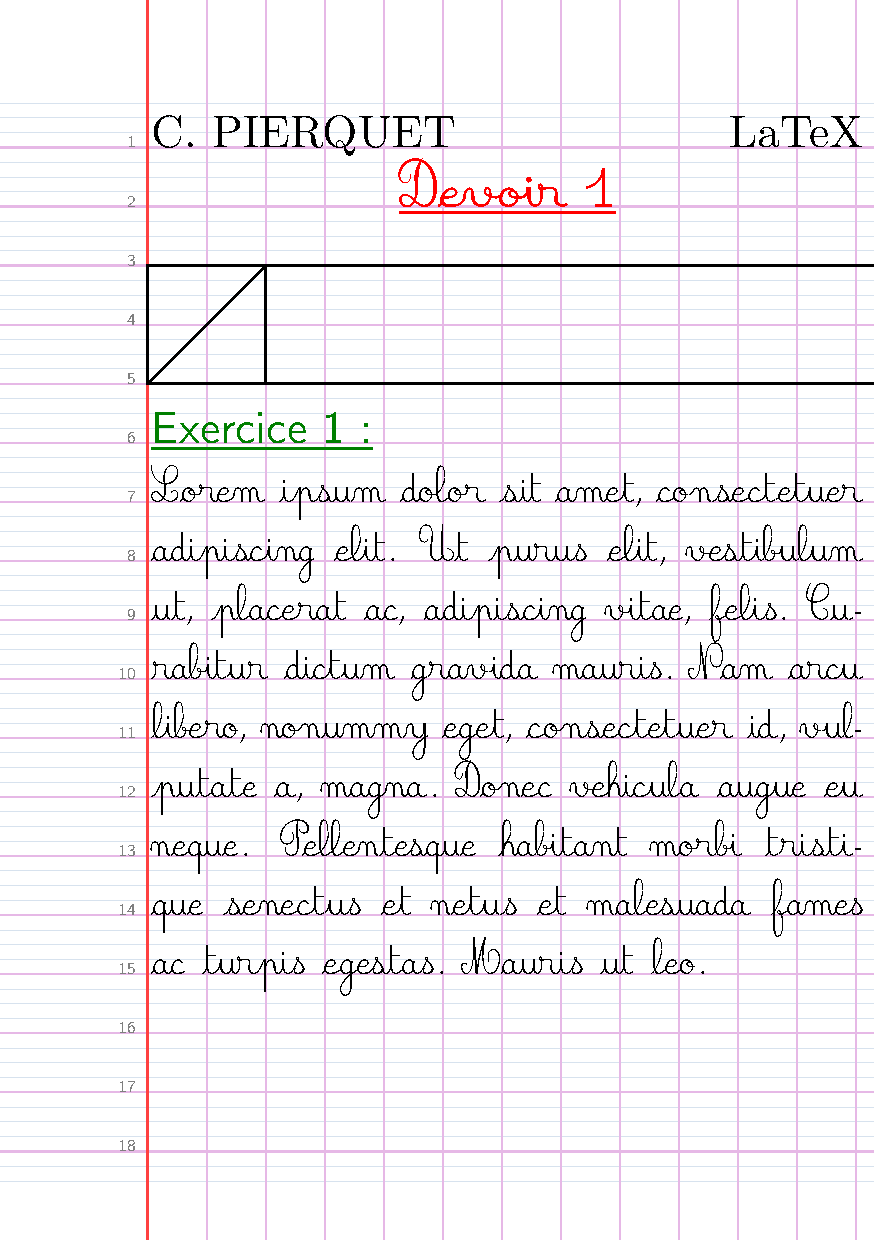
\includegraphics{WriteOnGrid-Seyes-A5.pdf}
}

\pagebreak

\section{Pages type 5x5 et College Ruled}

\subsection{Fonctionnement global}

Les commandes, méthodes et remarques de la section précédente sur les grilles Seyes peuvent être adaptées pour les grilles de type 5x5 et College Ruled.

\subsection{Commandes et environnements}

Les commandes et environnements sont suffixées différemment, mais le reste est identique !

\begin{PresentationCode}{listing only}
\pagestyle{empty}

\begin{PleinePageCinqCinq}[options]
	\LignePapierCinqCinq[options]<alignement>(ajustement){texte}
	\CadreNoteCinqCinq[hauteur]{numligne}
	\ParagraphePapierCinqCinq[options]<alignement>(ajustement){texte}
\end{PleinePageSeyes}
\end{PresentationCode}

\begin{PresentationCode}{listing only}
\pagestyle{empty}

\begin{PleinePageRuled}[options]
	\LignePapierRuled[options]<alignement>(ajustement){texte}
	\CadreNoteRuled[hauteur]{numligne}
	\ParagraphePapierRuled[options]<alignement>(ajustement){texte}
\end{PleinePageSeyes}
\end{PresentationCode}

{\small\faBomb} Pour les pages complètes 5x5, il est possible d'utiliser les clés \Cle{MargeG} et \Cle{MargeH} qui valent \Cle{auto} par défaut (adaptées au format du papier), mais elles peuvent être définies manuellement, avec les \textbf{contraintes} suivantes (pour un affichage correct sur les lignes, pour le moment\ldots) :

\begin{itemize}
	\item \Cle{MargeG} doit valoir $0.2$ ou $0.7$ ou $1.2$ ou $1.7$ etc
	\item \Cle{MargeH} doit valoir $0.3$ ou $0.8$ ou $1.3$ ou $1.8$ etc
\end{itemize}

\subsection{Exemples}

Les exemples des pages suivantes ont été obtenus de la même manière que celui de la pleine page Seyes, il \textit{suffit} d'adapter les commandes et environnements avec le bon suffixe.

\begin{PresentationCode}{listing only}
\pagestyle{empty}

\begin{PleinePageCinqCinq}[NumLignes,MargeG=2.7,MargeH=2.3]
	\LignePapierCinqCinq[Echelle=1.25,Ligne=1]{C. PIERQUET \hfill LaTeX}
	\LignePapierCinqCinq[Echelle=1.25,Ligne=3,Couleur=red]<center>{\underline{\cursive\bfseries Devoir 2}}
	\CadreNoteCinqCinq{4}
	\LignePapierCinqCinq[Echelle=1.25,Ligne=9,Couleur=green!50!black]{\sffamily\underline{Exercice 1 :}}
	%echelle de 1.25 et espacement de 10mm (2 lignes) := calcul 10/1.25 pour l'espacement
	\ParagraphePapierCinqCinq[Ligne=11,Echelle=1.25,Espacement=\fpeval{10/1.25}]{\cursive\lipsum[1]}
	\ParagraphePapierCinqCinq[Ligne=38]
	{%
		On essaye avec des maths $1+\frac12=\frac32$ en mode ligne avec des lignes assez longues pour voir
		ce que ça peut donner\ldots Et une intégrale $\int_0^1 2x dx = 1$.\\On essaye en passant à la ligne !!!
	}
\end{PleinePageCinqCinq}
\end{PresentationCode}

\begin{PresentationCode}{listing only}
\pagestyle{empty}

\begin{PleinePageRuled}[NumLignes]
	\LignePapierRuled[Echelle=1.25,Ligne=1]{C. PIERQUET \hfill LaTeX}
	\LignePapierRuled[Echelle=1.25,Ligne=2,Couleur=red]<center>{\underline{\cursive\bfseries Devoir 3}}
	\CadreNoteRuled{3}
	\LignePapierRuled[Echelle=1.25,Ligne=8,Couleur=green!50!black]{\sffamily\underline{Exercice 1 :}}
	%echelle de 1.33 et espacement de 9mm (1 ligne) := calcul 9/1.33 pour l'espacement
	\ParagraphePapierRuled[Ligne=9,Echelle=1.33,Espacement=\fpeval{9/1.25}]{\cursive\lipsum[1]}
	\ParagraphePapierRuled[Ligne=28]
	{%
		On essaye avec des maths $1+\frac12=\frac32$ en mode ligne avec des lignes assez longues pour voir
		ce que ça peut donner\ldots Et une intégrale $\int_0^1 2x dx = 1$.\\On essaye en passant à la ligne !!!
	}
\end{PleinePageRuled}
\end{PresentationCode}

\pagebreak

\pagestyle{empty}

\begin{PleinePageCinqCinq}[NumLignes,MargeG=2.7,MargeH=2.3]
	%marges pour illustrer
	\draw[thick,teal,<->,>=latex] ([shift={(-2.7,1.5)}]CinqCinqOrigine) --++ (2.7,0) node[midway,below,font=\small\ttfamily] {MargeG} ;
	\draw[thick,orange,<->,>=latex] ([shift={(-0.5,0)}]CinqCinqOrigine) --++ (0,2.3) node[midway,right,font=\small\ttfamily] {MargeH} ;
	%back to normal
	\LignePapierCinqCinq[Echelle=1.25,Ligne=1]{C. PIERQUET \hfill LaTeX}
	\LignePapierCinqCinq[Echelle=1.25,Ligne=3,Couleur=red]<center>{\underline{\cursive\bfseries Devoir 2}}
	\CadreNoteCinqCinq{4}
	\LignePapierCinqCinq[Echelle=1.25,Ligne=9,Couleur=green!50!black]{\sffamily\underline{Exercice 1 :}}
	%echelle de 1.25 et espacement de 10mm (2 lignes) := calcul 10/1.25 pour l'espacement
	\ParagraphePapierCinqCinq[Ligne=11,Echelle=1.25,Espacement=\fpeval{10/1.25}]{\cursive\lipsum[1]}
	\ParagraphePapierCinqCinq[Ligne=38]
	{%
		On essaye avec des maths $1+\frac12=\frac32$ en mode ligne avec des lignes assez longues pour voir
		ce que ça peut donner\ldots Et une intégrale $\int_0^1 2x dx = 1$.\\On essaye en passant à la ligne !!!
	}
\end{PleinePageCinqCinq}

\pagebreak

\pagestyle{empty}

\begin{PleinePageRuled}[NumLignes]
	\LignePapierRuled[Echelle=1.25,Ligne=1]{C. PIERQUET \hfill LaTeX}
	\LignePapierRuled[Echelle=1.25,Ligne=2,Couleur=red]<center>{\underline{\cursive\bfseries Devoir 3}}
	\CadreNoteRuled{3}
	\LignePapierRuled[Echelle=1.25,Ligne=8,Couleur=green!50!black]{\sffamily\underline{Exercice 1 :}}
	\ParagraphePapierRuled[Ligne=9,Echelle=1.33,Espacement=\fpeval{9/1.33}]{\cursive\lipsum[1]}
	\ParagraphePapierRuled[Ligne=28]
	{%
		On essaye avec des maths $1+\frac12=\frac32$ en mode ligne avec des lignes assez longues pour voir
		ce que ça peut donner\ldots Et une intégrale $\int_0^1 2x dx = 1$.\\On essaye en passant à la ligne !!!
	}
\end{PleinePageRuled}

\pagebreak

\section{Historique}

\verb|v0.1.7|~:~~~~Option pour régler la marge pour les \textsf{PleinePageCinqCinq}

\verb|v0.1.6|~:~~~~Possibilité de déterminer automatiquement L\&C en fonction de la place restante.

\verb|v0.1.5|~:~~~~Possibilité de spécifier la réglure pour les quadrillages de type \textsf{Seyes} + meilleure gestion des paragraphes.

\phantom{\texttt{v0.1.5}}~:~~~~Amélioration de la gestion des paragraphes en mode \textsf{pleine page}.

\verb|v0.1.4|~:~~~~Modification de la gestion des couleurs (\texttt{xcolor} n'est plus chargé avec \textsf{[table,svgnames]})

\verb|v0.1.3|~:~~~~Ajout d'une commande pour afficher (sans écrire dessus) une grille

\verb|v0.1.2|~:~~~~Ajustement au niveau des couleurs + raccourcis couleurs par défaut

\verb|v0.1.1|~:~~~~Meilleure gestion des couleurs du quadrillage + Ajout pages complètes

\verb|v0.1.0|~:~~~~Version initiale

\end{document}